\documentclass[a4paper,10pt]{article}

% Hier die Nummer des Blatts und Autoren angeben.
\newcommand{\blatt}{1}
\newcommand{\autor}{Frederik Wille}

\usepackage{hci}

\begin{document}
% Seitenkopf mit Informationen
\kopf

\renewcommand{\figurename}{Figure}

\aufgabe{1}
\begin{enumerate}

\item Ein Produkt, das den Inuit-Indianern die Navigation entlang der Küste erleichtern soll, muss sich den ihnen und ihrem Umfeld anpassen.\\
Ein elektronisches Gerät muss als Beispiel vorallem der extremen Kälte und dem Wasser widerstehen. Außerdem muss eine lange Akkulaufzeit gewährt sein, damit die Inuit nicht bei ihren gewohnten Abläufen gestört werden.\\
Um das Problem zulösen benötigt ein Gerät die eigene Position und dazu passende Kartendaten. Es muss den Inuits am besten während der Fahrt den Weg weisen und dabei weder Stören noch die Bedienung mit einer Hand erfordern.
\item
\begin{figure}[ht]
\centering 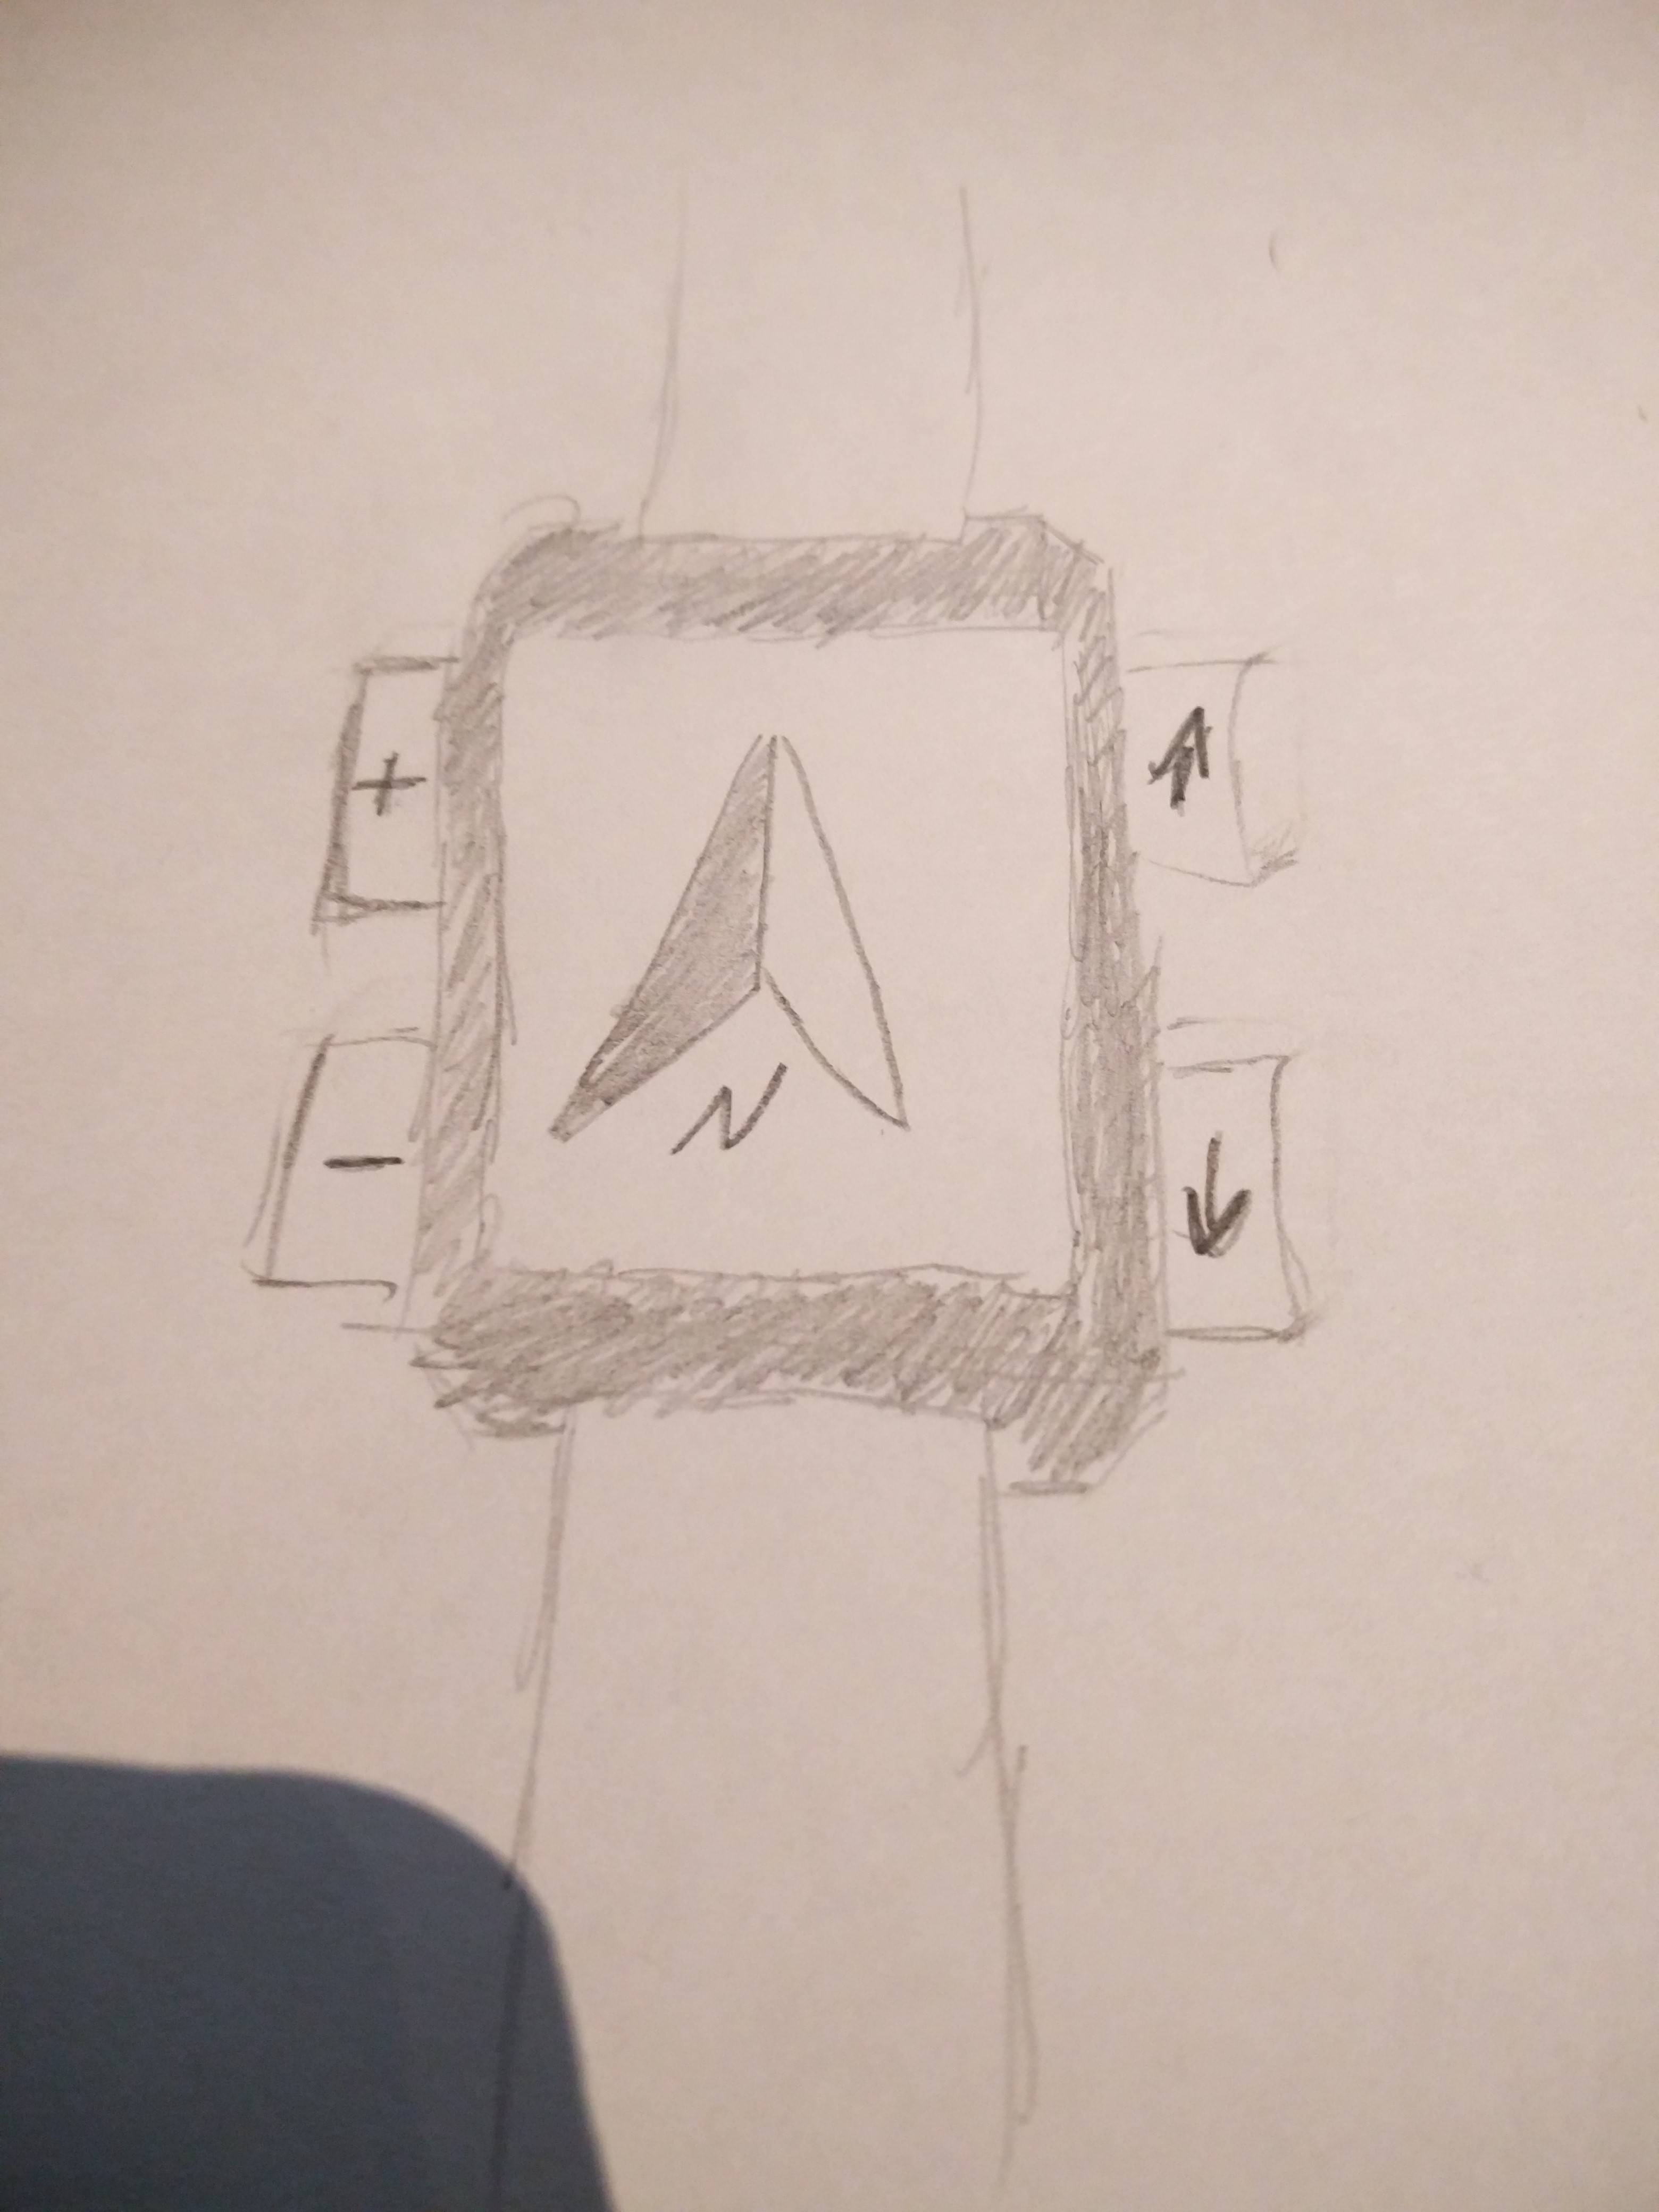
\includegraphics[width=0.4\textwidth]{images/uhr.jpg}
% \caption{}
\label{fig:wwu_logo}
\end{figure}

\item Angeboten wird eine Art von Smartwatch, die im Vergleich zu bekannten Angeboten auf Bluetooth verzichtet und stattdessen ein GPS-Modul verbaut hat. Wie bereits erhältliche Produkte ist diese Wasserdicht und sollte zusätzlich gegen die eisigen Temperaturen gedämmt werden. Auch das Armband ist so stabil wie möglich, ohne dabei Unangenehm am Arm zusein.\\
Auf einem kleinen Display kann sowohl die nähere Umgebung als auch eine Übersicht über die aktuelle Position angezeigt werden. Das Display sollte möglichst hoch aufgelösend sein, um die Umgebung best möglich darzustellen. Ein Touchdisplay ergibt auf Grund des Tragens von Handschuhen keinen Sinn, stattdessen werden gut erreichbare Knöpfe angebracht. Mithilfe der Knöpfe auf der linken Seite der Uhr kann man auf der Karte zoomen. Mit den rechten Knöpfen kann auf einen Kompass, eine Richtungsanzeige zu einem angegebenem Ziel und zu potentiell weiteren Anzeigen gewechselt werden. Sowohl Kompass als auch Richtungsanzeige können auch über die Karte eingeblendet werden. Durch Vibrationen kann haptisch eine Richtung zum Ziel gezeigt werden. Der Informationen wie der zeitbasiert berechnete Gezeitenwechsel können ebenfalls durch Vibration und Anzeige auf dem Display signalisiert werden.\\
Einstellen der Uhr und Aufladen erfolgen durch einen Anschluss auf der Rückseite. Dazu gibt es ein Kabel das zu dem USB Standard kompatibel ist.\\
Durch den Verzicht auf Bluetooth und eine Toucheingabe und ohne Anforderung an einen starken Prozessor kann im Vergleich viel Stromverbrauch eingespart werden. Damit sollte der verbaute Akku einige Tage halten und kann bei Sonnenlicht durch Solarzellen auf den freien Flächen der Kajaks und an Land aufgeladen werden. \\
Dies soll erst einmal als Grundausstattung stehen und kann, wenn es Größe und Akkuleistung zulassen, durch Funkverbindungen zum Empfangen aktueller Strömungs- und Wetterinformation ergänzt werden. Auch können Druck- und Temperatursensoren angebracht werden, die als lokale Werte ausgewertet und angezeigt werden können.

\end{enumerate}
\begin{figure}[ht]
\centering 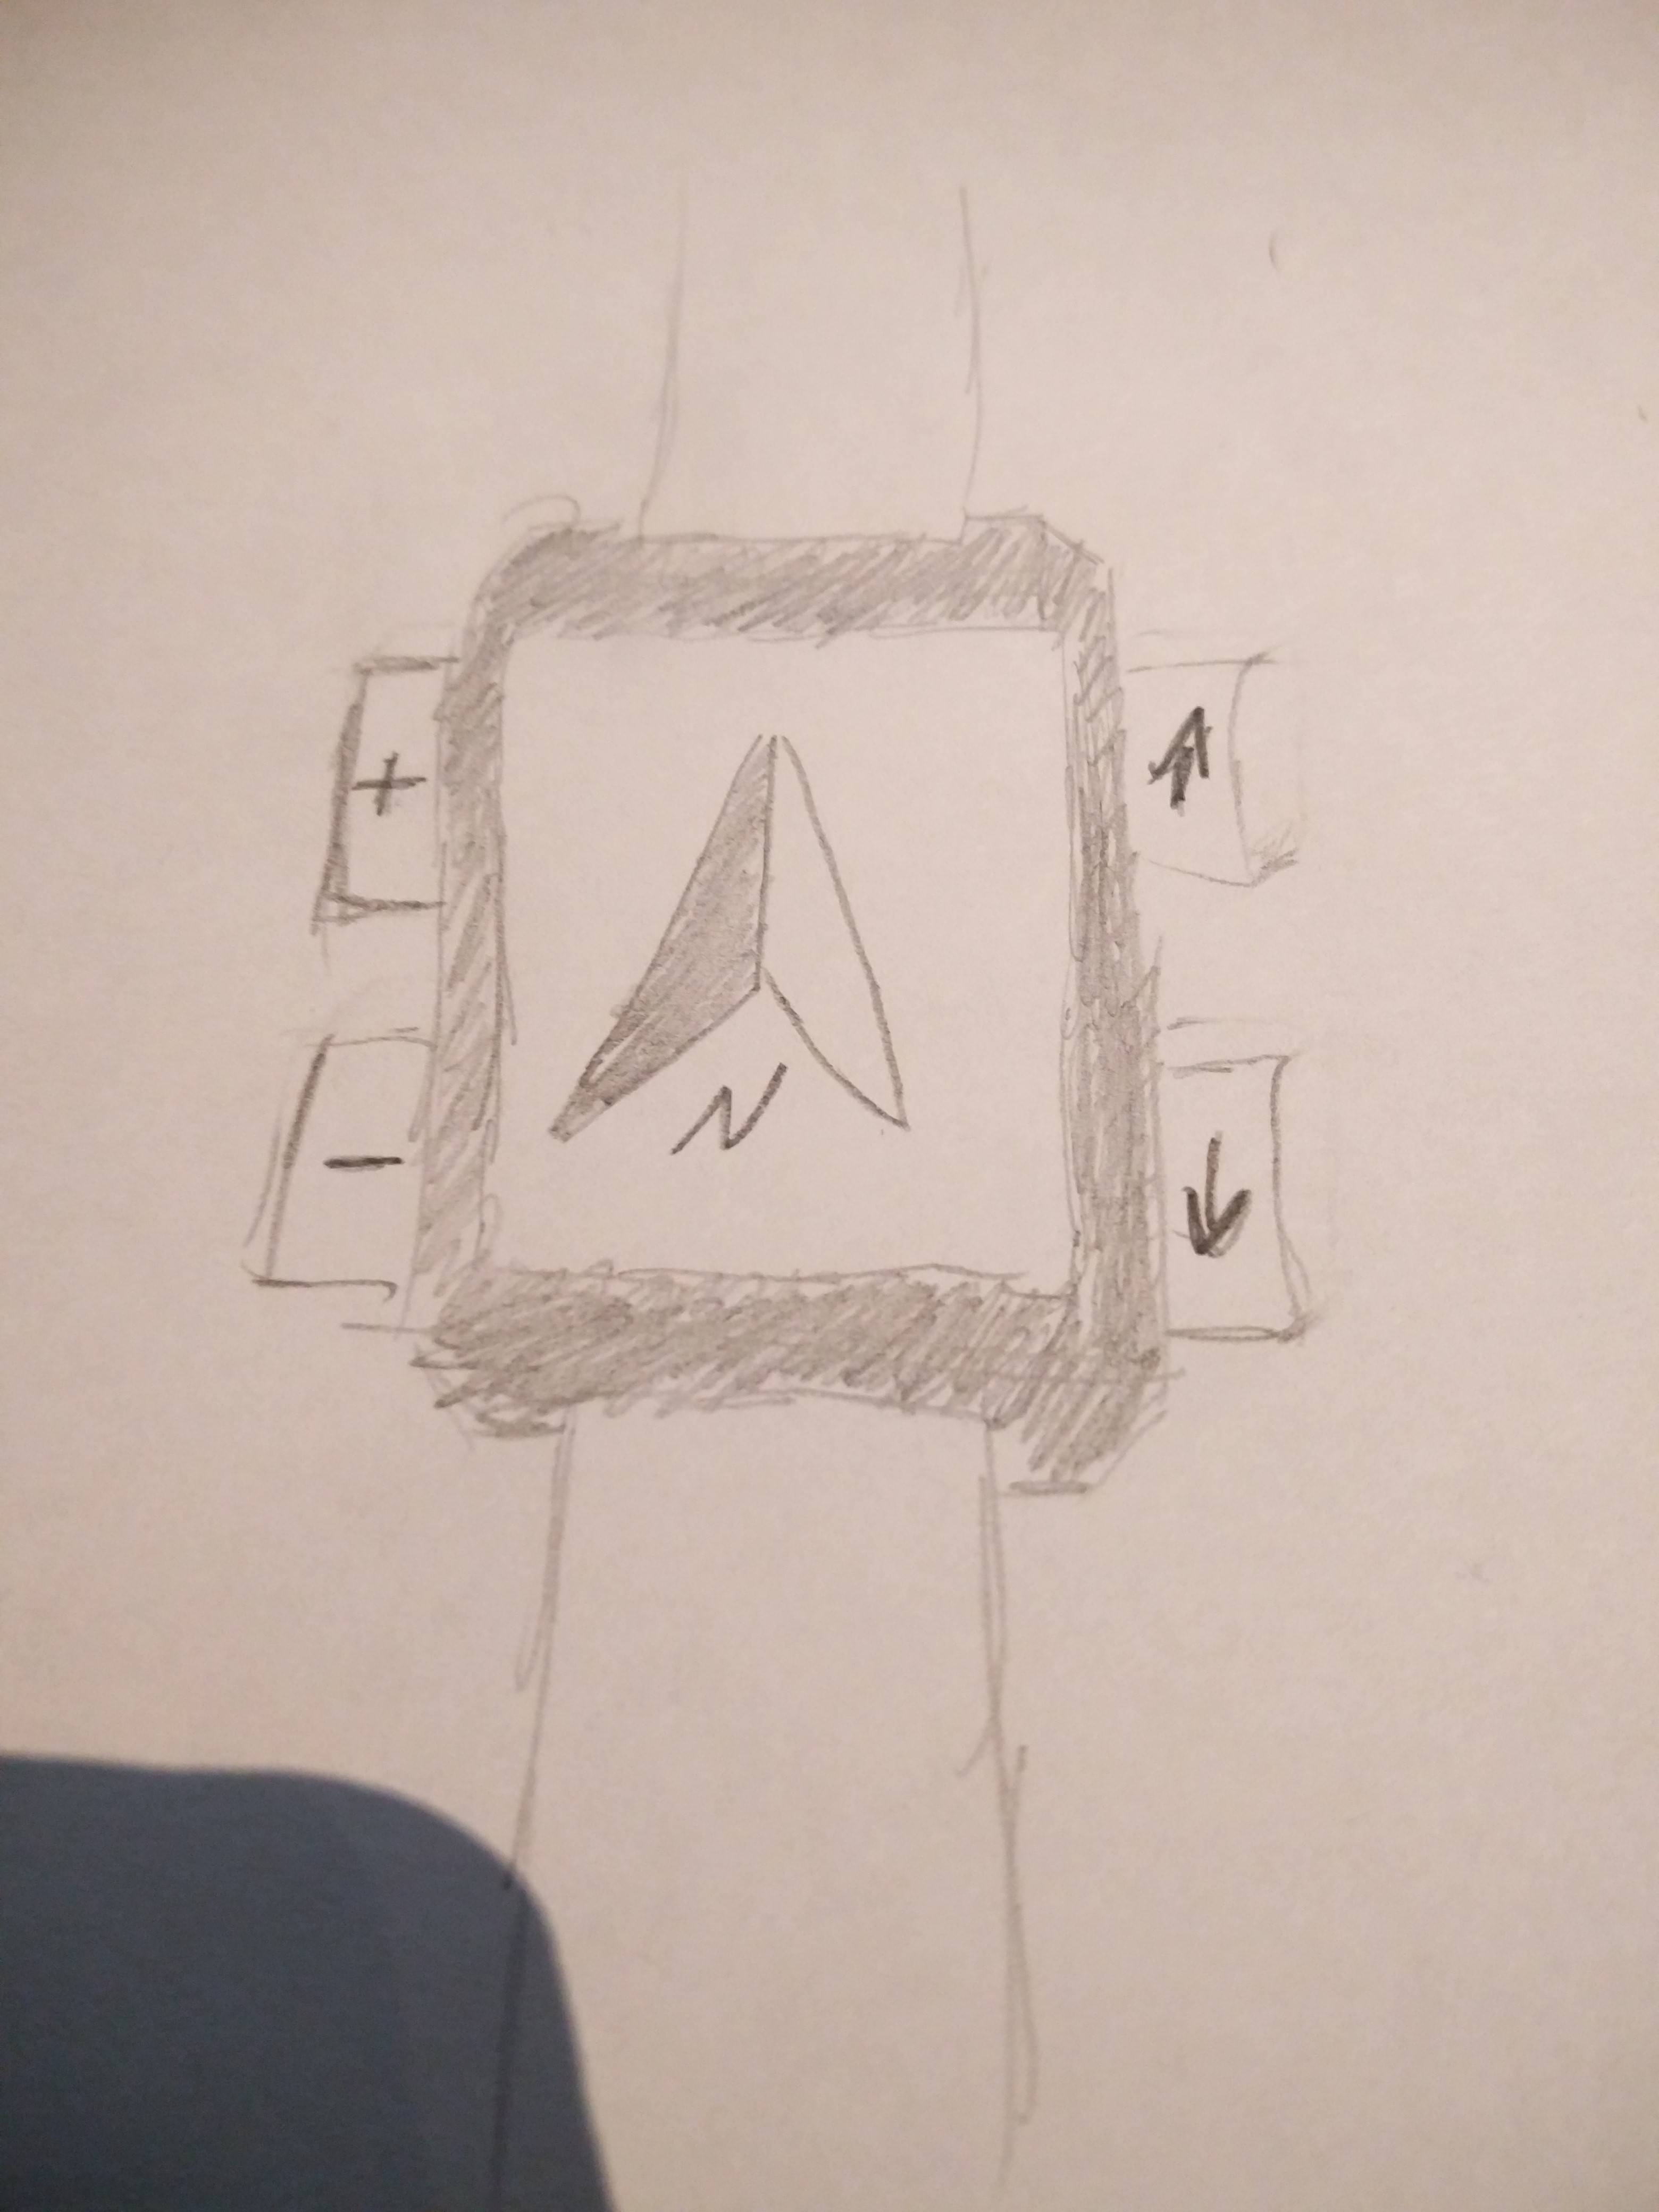
\includegraphics[width=1.0\textwidth]{images/uhr.jpg}
% \caption{Human-Computer Interaction}
\label{fig:wwu_logo}
\end{figure}\begin{figure}[ht]
\centering 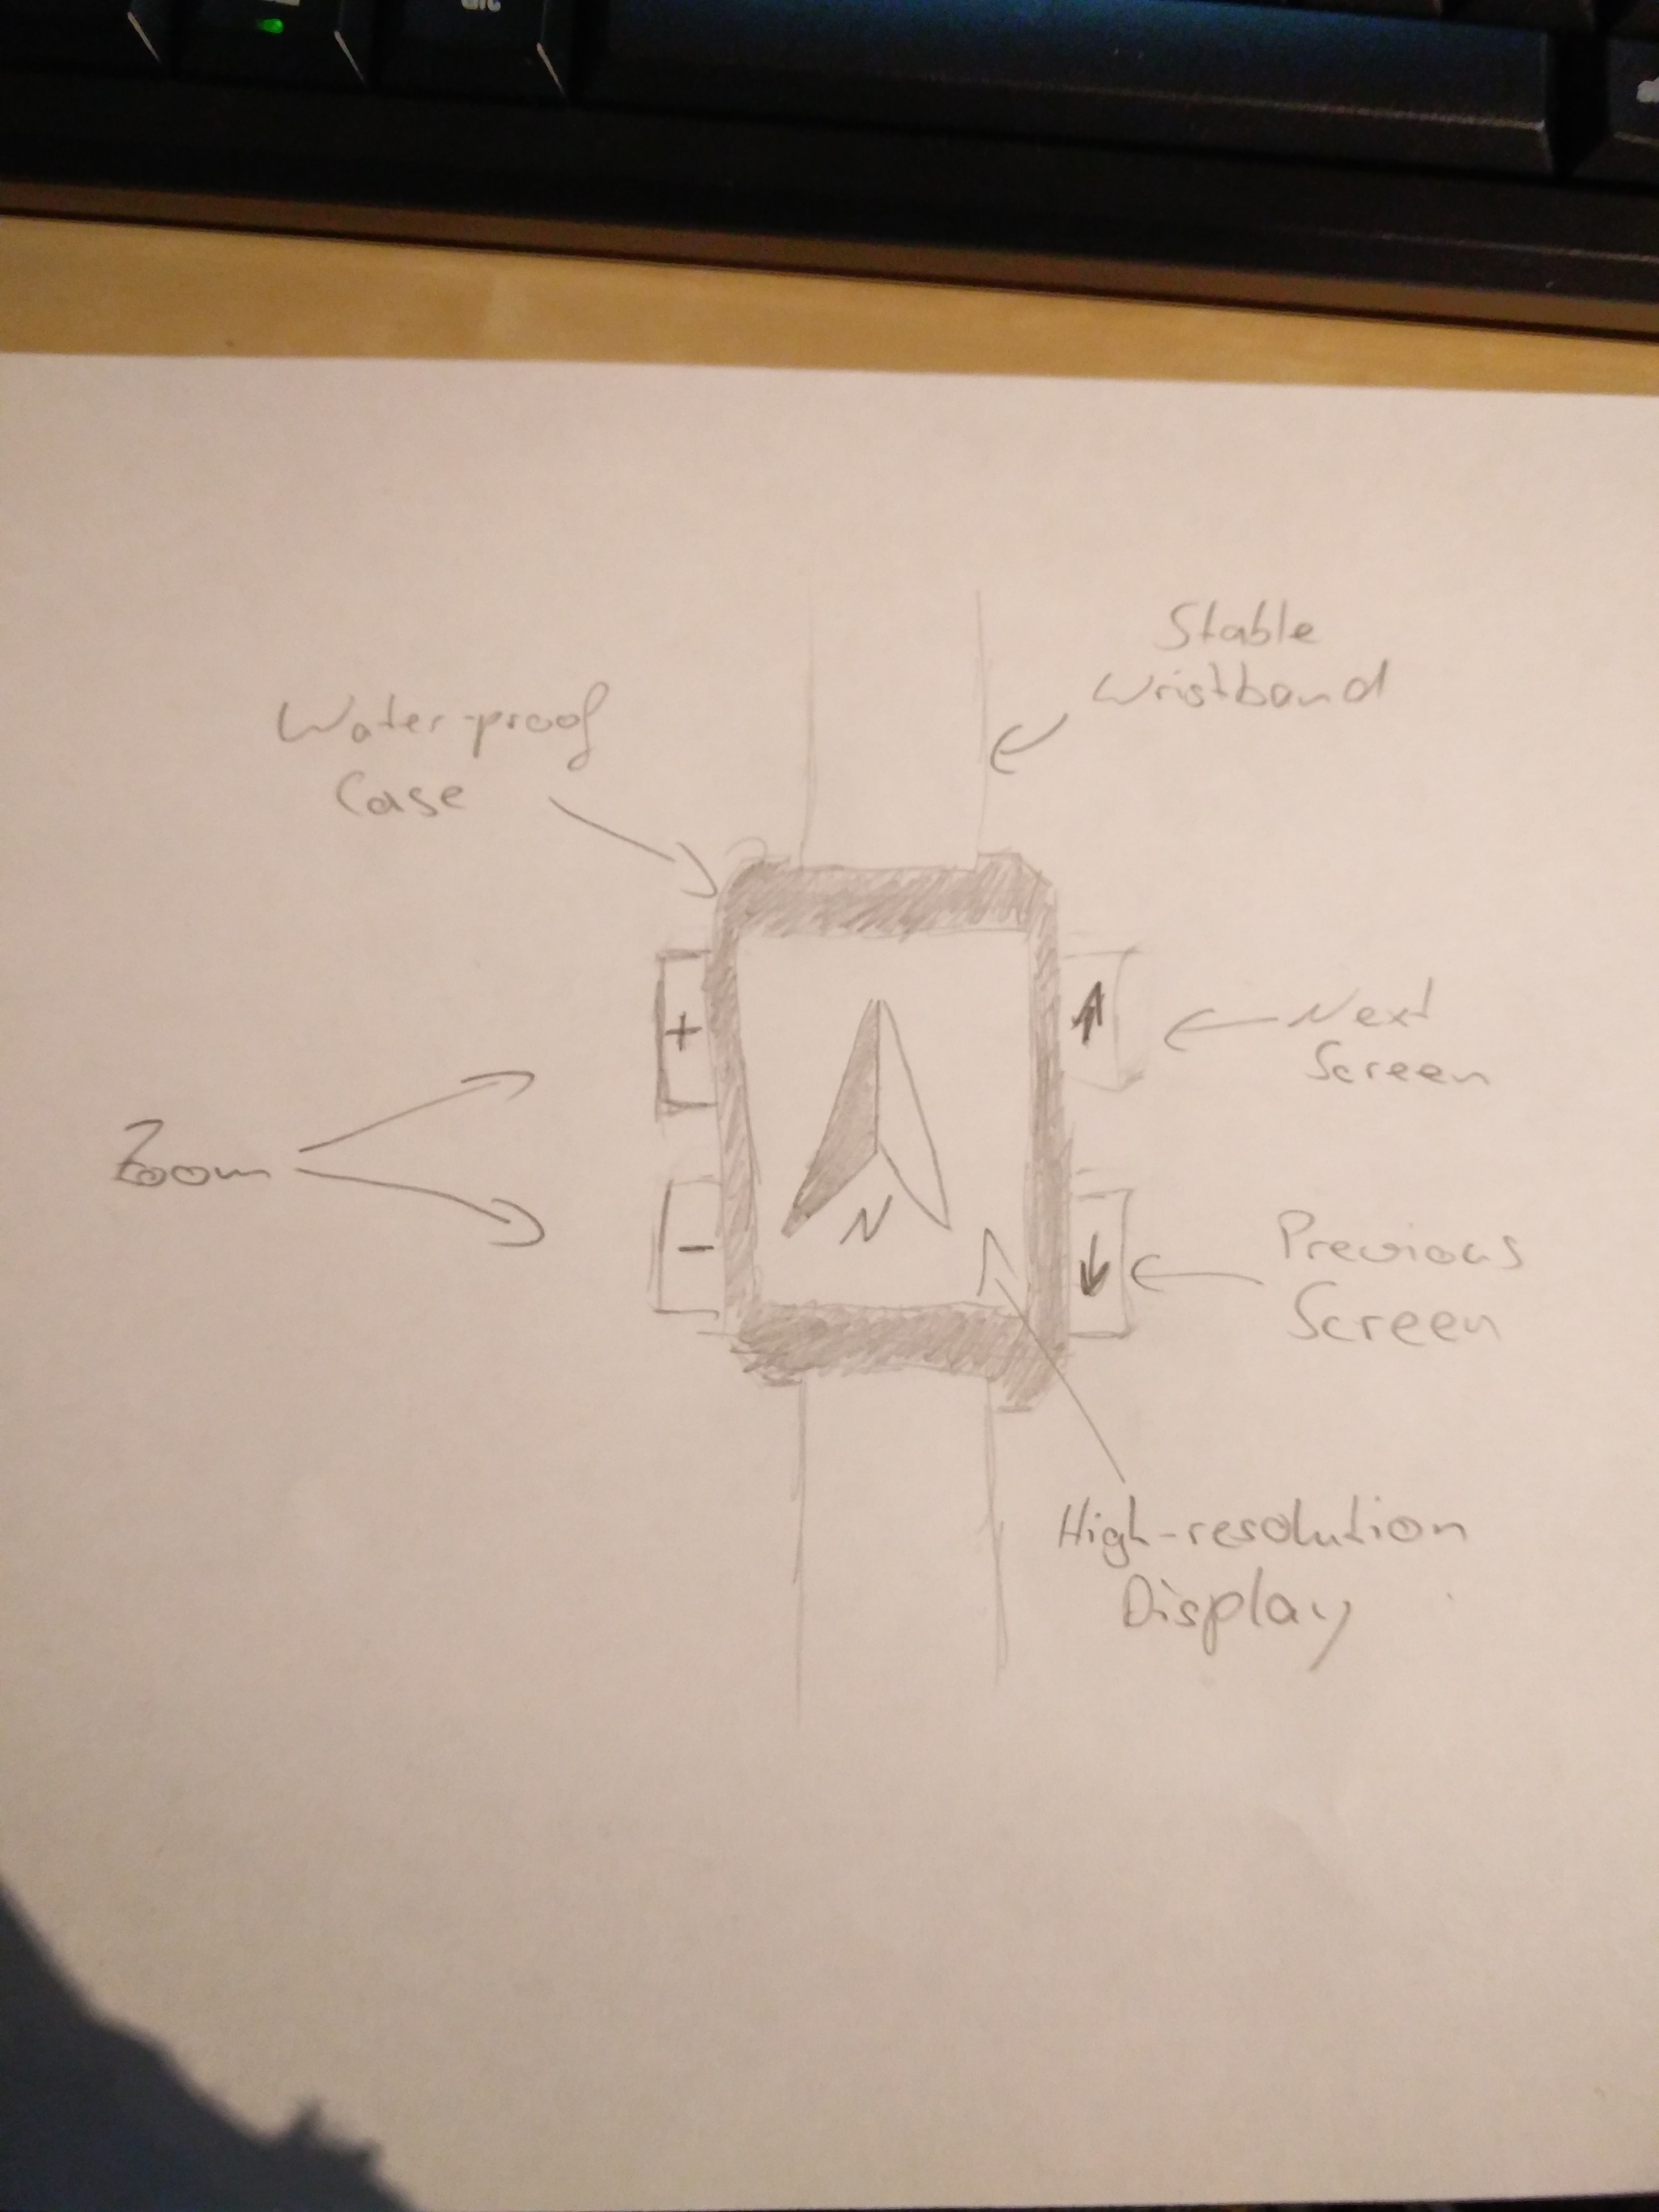
\includegraphics[width=1.0\textwidth]{images/uhr2.jpg}
% \caption{Human-Computer Interaction}
\label{fig:wwu_logo}
\end{figure}
\end{document}
